%% ======================================================================
%% 08_operation.tex -- 7. Instrucciones de operacion
%% ======================================================================
\section{Instrucciones de operación}
\label{sec:operation}

\begin{figure}[!htbp]
  \centering
  \begin{subfigure}[b]{0.52\textwidth}\centering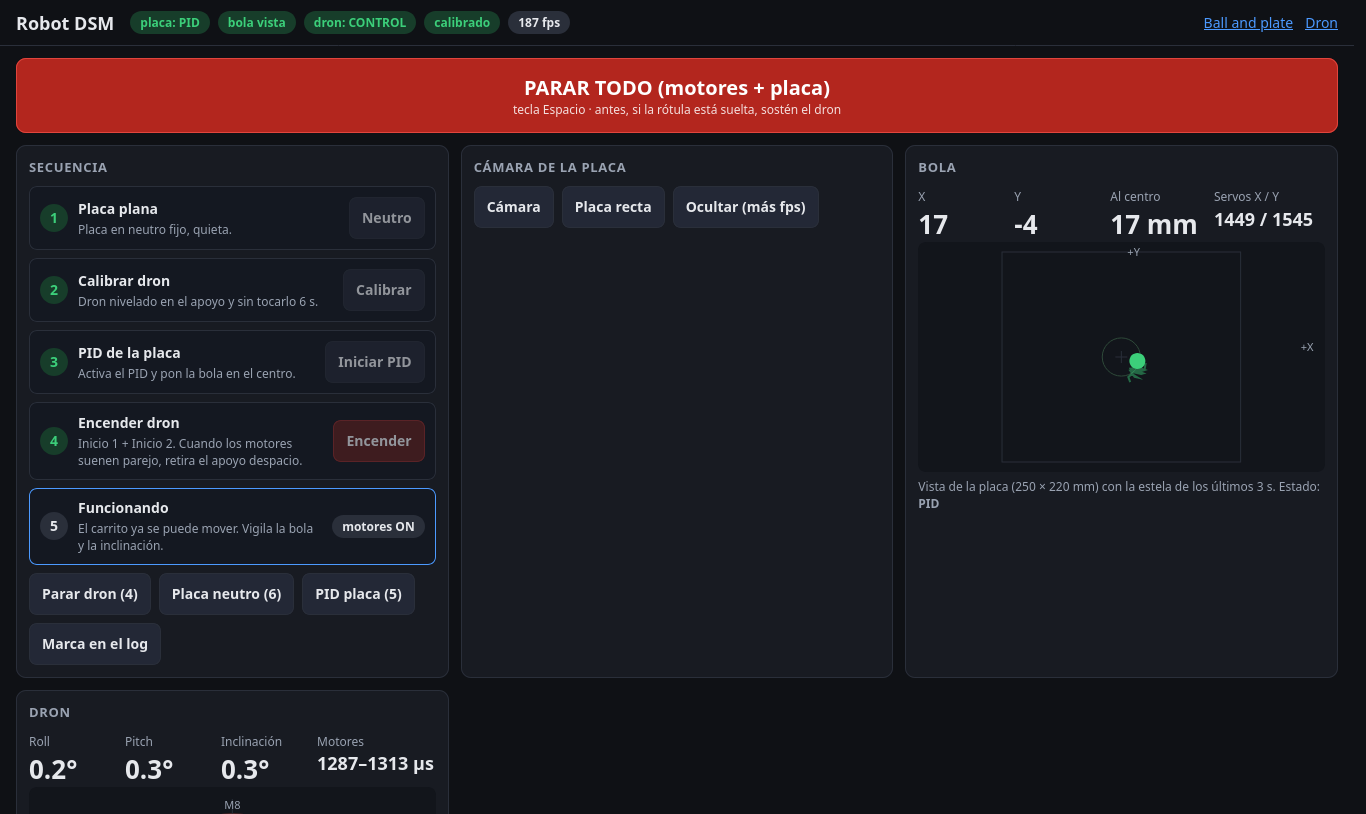
\includegraphics[width=\linewidth]{figures/ui_robot_page.png}\caption{Página web \texttt{/robot} servida por la Pi.}\end{subfigure}\hfill
  \begin{subfigure}[b]{0.45\textwidth}\centering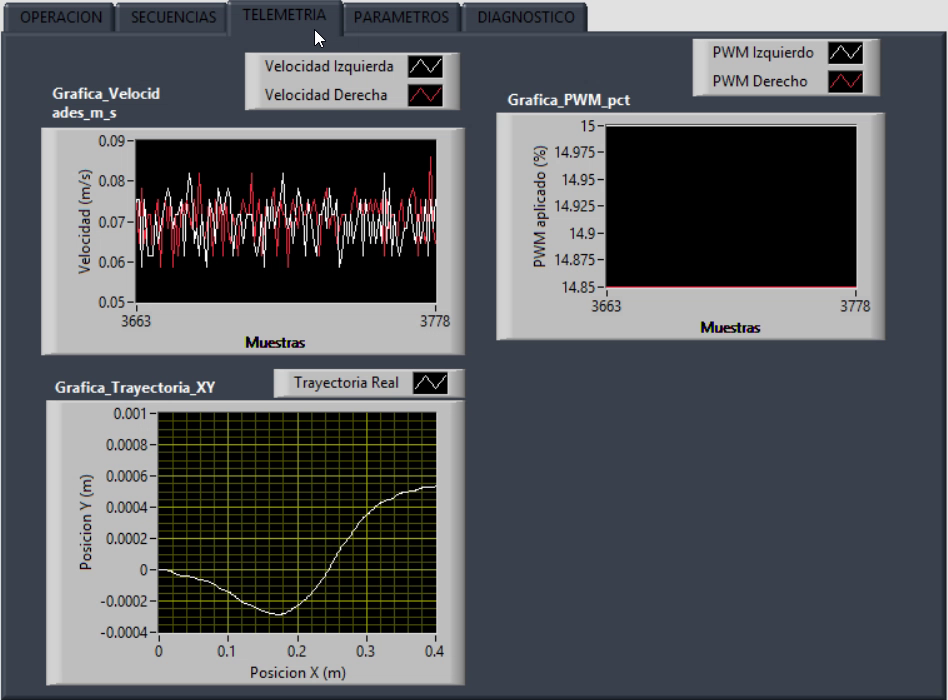
\includegraphics[width=\linewidth]{figures/ui_labview_telemetry.png}\caption{Pestaña de telemetría de LabVIEW (myRIO).}\end{subfigure}
  \caption{Interfaces del operador. La página web muestra el estado del plato, de la bola y del dron, una secuencia guiada de arranque y un botón de PARAR TODO (también la barra espaciadora); el panel de LabVIEW muestra las velocidades de las ruedas, el PWM y la trayectoria $x$--$y$.}
  \label{fig:ui}
\end{figure}

\paragraph{Requisitos previos}
\begin{itemize}
  \item baterías cargadas: las dos LiPo a \SI{12.6}{\volt} en reposo y con menos de \SI{0.05}{\volt} de diferencia entre sí, la NiMH, los dos packs 18650 y el power bank;
  \item hélices revisadas y ajustadas;
  \item guía libre, con ambos topes en su lugar;
  \item una laptop o un celular en la misma red Wi-Fi que la Pi;
  \item dos operadores: uno en la página web, con la barra espaciadora como parada inmediata, y otro mirando el robot con el hongo de emergencia SB1 a mano;
  \item lentes de seguridad para todas las personas a menos de \SI{2}{\metre}.
\end{itemize}

\paragraph{Secuencia de arranque}
La Fig.~\ref{fig:fsm_dron} resume la máquina de estados del firmware v11 del octocóptero que gobierna el arranque, el vuelo en guía y los cortes de seguridad.
\begin{enumerate}
  \item Con SB1 pulsado, encender la lógica (SW1). \texttt{arrancar.sh} lanza \texttt{seguidor.py} y lo reinicia si se detiene. Esperar a que la NodeMCU arranque: así los pulsos que emiten GPIO5 y GPIO14 durante el arranque no llegan a ESC energizados.
  \item Encender la myRIO y lanzar el VI de LabVIEW. El módulo UART debe mostrar la posición recibida de la bola y los ángulos del dron (Fig.~\ref{fig:ui}b).
  \item En \texttt{/robot}:
  \begin{enumerate}[label=\alph*.]
    \item poner el plato en \emph{Neutro};
    \item con el dron nivelado y quieto, pulsar \emph{Calibrar} y esperar 5\,s hasta ``CAL OK'';
    \item pulsar \emph{Iniciar PID} con la bola cerca del centro.
  \end{enumerate}
  \item Medir la tensión en reposo de las dos LiPo, anotarla y conectarlas. Soltar SB1 (cierran K1--K4). Pulsar \emph{Armar e iniciar motores}: el colectivo sube en rampa a \SI{1300}{\micro\second} (ralentí) y el lazo de actitud queda activo.
  \item \textbf{Modo banco} (base en movimiento, dron en ralentí). Mover la base desde LabVIEW con una orden manual, un objetivo de distancia, el giro de \SI{360}{\degree}, ir a un punto o una secuencia cargada.
  \item \textbf{Modo rampa} (propuesto, Sección~\ref{sec:porquedron}). Antes de la rampa, subir el colectivo con \emph{Subir} hasta 1450--\SI{1550}{\micro\second} ($f\approx0.35$--0,55): el módulo sigue apoyado, pero los rotores sostienen parte de su peso. Bajar a \SI{1300}{\micro\second} al terminar la subida. Por encima de \SI{1500}{\micro\second} el firmware limita el tramo a \SI{90}{\second}.
  \item \textbf{Vuelo en guía.} Pulsar \emph{Flotar}: el colectivo sube a \SI{25}{\micro\second\per\second}, a \SI{8}{\micro\second\per\second} por encima de \SI{1650}{\micro\second}, hasta \SI{1750}{\micro\second}. Si el módulo no despega, usar \emph{Subir} ($+$\SI{25}{\micro\second}) y anotar el colectivo de despegue; si pasa de \SI{1825}{\micro\second}, aterrizar y cambiar las baterías (Sección~\ref{sec:bateria}). Usar \emph{Subir/Bajar} ($\pm$\SI{25}{\micro\second}) y \emph{Mantener}; terminar con \emph{Aterrizar}, que baja a \SI{60}{\micro\second\per\second}.
\end{enumerate}

\begin{figure}[!htbp]
\centering
\begin{tikzpicture}[font=\footnotesize, >=Latex,
  st/.style={draw, rounded corners=3pt, align=center, minimum height=11.5mm, inner xsep=3.5pt, inner ysep=3pt, line width=0.7pt},
  stOff/.style={st, draw=pGris!90!black, fill=pGris!12, line width=1.1pt, text width=2.80cm},
  stPre/.style={st, draw=pOcre, fill=pOcre!10, text width=2.55cm},
  stVis/.style={st, draw=pAzul, fill=pAzul!8, text width=2.65cm},
  stArm/.style={st, draw=pOcre, fill=pOcre!12, text width=2.45cm},
  stRmp/.style={st, draw=pAzul, fill=pAzul!10, text width=2.65cm},
  stSub/.style={st, draw=pVerde!90!black, fill=white, minimum height=15mm, text width=4.85cm},
  stCut/.style={st, draw=pRojo, fill=pRojo!8, align=left, text width=4.68cm, line width=0.85pt, inner xsep=3pt, inner ysep=2pt, font=\footnotesize\linespread{0.95}\selectfont},
  tr/.style={->, line width=0.8pt, pAzul!90!black, rounded corners=2.5pt},
  trG/.style={->, line width=0.8pt, pVerde!85!black, rounded corners=2.5pt},
  trR/.style={->, line width=0.95pt, pRojo, rounded corners=2.5pt},
  lbl/.style={font=\footnotesize, align=center, inner sep=1.5pt}]

  % ---- Nivel 1: Preparacion (y = 0.00, ancho total 0.00..13.50 cm <= 13.74 cm)
  \node[stPre] (cal) at (1.42, 0.00) {\textbf{CAL}\\ \SI{5}{\second} inmóvil\\ (1000 muestras)};
  \node[stOff] (off) at (6.75, 0.00) {\textbf{DESARMADO}\\ (\texttt{OFF}, \SI{1000}{\micro\second})};
  \node[stVis] (vis) at (12.02, 0.00) {\textbf{VISTA}\\ (\texttt{PREVIEW},\\ \SI{1000}{\micro\second})};

  % Flecha de inicio hacia DESARMADO
  \fill[pGris!90!black] (6.75, 1.20) circle (0.08);
  \draw[->, thick, pGris!90!black] (6.75, 1.13) -- node[right=2pt]{\texttt{setup()}} (off.north);

  % Transiciones Nivel 1 (huecos 2.85..5.20 = 2.35 cm y 8.30..10.55 = 2.25 cm)
  \draw[tr]  ([yshift=2.4mm]off.west) -- node[lbl, above=1.5pt]{\texttt{cal} ($\ge\SI{4}{\second}$)} ([yshift=2.4mm]cal.east);
  \draw[tr]  ([yshift=-2.4mm]cal.east) -- node[lbl, below=1.5pt]{CAL OK\\ o rechazada} ([yshift=-2.4mm]off.west);
  \draw[tr]  ([yshift=2.4mm]off.east) -- node[lbl, above=1.5pt]{\texttt{vista} (cal.)} ([yshift=2.4mm]vis.west);
  \draw[trR] ([yshift=-2.4mm]vis.west) -- node[lbl, below=1.5pt, pRojo]{\texttt{parar} / \texttt{!}} ([yshift=-2.4mm]off.east);

  % ---- Nivel 2: Seguridad (izq), ARMADO (centro), RAMPA (der) (y = -3.65)
  \node[stCut] (cut) at (2.48, -3.72) {%
    \textbf{\textcolor{pRojo}{Cortes de seguridad}}\\
    $\bullet$ \texttt{parar}, \texttt{!} u orden inválida\\
    $\bullet$ inclinación $\ge\SI{12}{\degree}$\\
    $\bullet$ guiñada $\ge20^\circ$$^\ast$\\
    $\bullet$ giro $\ge35^\circ$/s$^\ast$\\
    $\bullet$ error I$^2$C o PWM\\
    $\bullet$ IMU lenta; ciclo $>\SI{30}{\milli\second}$\\
    {\scriptsize $^\ast$en ralentí: ventana $\pm20^\circ$, $120^\circ$/s}};
  \node[stArm] (arm) at (7.45, -3.65) {\textbf{ARMADO}\\ espera \texttt{iniciar}\\ (límite \SI{10}{\second})};
  \node[stRmp] (rmp) at (12.02, -3.65) {\textbf{RAMPA}\\ $1000\to\SI{1300}{\micro\second}$\\ ($+5\us/\SI{20}{\milli\second}$)};

  % Transiciones Nivel 1 <-> Nivel 2 (espacio vertical -0.65..-2.55)
  % DESARMADO y VISTA comparten la transicion arm BANCO_FIJO hacia ARMADO
  \draw[tr]  ([xshift=7mm]off.south) -- node[lbl, right=2pt, pos=0.62, align=left]{\texttt{arm BANCO\_FIJO}\\ (cal., $\le\SI{4}{\degree}$, $\le\SI{5}{\degree\per\second}$)} (arm.north);
  \draw[tr]  (vis.south) -- ++(0,-0.48) -| ([xshift=7mm]off.south |- 0,-1.35);
  % Timeout 10 s de ARMADO a DESARMADO (izquierda de arm.north)
  \draw[trR] ([xshift=-8mm]arm.north) -- node[lbl, left=2pt, pos=0.52, pRojo]{\SI{10}{\second}} ([xshift=-1mm]off.south);
  % Salida de Cortes hacia DESARMADO (etiqueta limpia sobre el codo, bien arriba de cut.north)
  \draw[trR] ([xshift=19mm]cut.north) -- (4.38,-1.52) -| ([xshift=-10mm]off.south);
  \node[lbl, pRojo, left=3pt, align=right] at (4.34, -1.68) {\texttt{stop()} $\to\SI{1000}{\micro\second}$};
  % Parada desde ARMADO hacia Cortes
  \draw[trR] (arm.west) -- node[lbl, above=1.5pt, pRojo]{\texttt{parar}} (cut.east |- arm.west);
  % ARMADO -> RAMPA (hueco 8.80..10.55 = 1.75 cm)
  \draw[tr]  (arm.east) -- node[lbl, above=1.5pt]{\texttt{iniciar}} node[lbl, below=1.5pt, align=center]{$<\SI{10}{\second}$\\ $\le\SI{4}{\degree}$} (rmp.west);

  % ---- Nivel 3: Contenedor CONTROL (y = -6.30..-13.25, ancho 0.00..13.50 cm)
  \node[stSub] (flt) at (2.82, -7.85) {\textbf{Flotar / colectivo manual}\\ \texttt{flotar} (\SI{1750}{\micro\second}), \texttt{maximo} (\SI{1950}{\micro\second})\\ \texttt{subir}/\texttt{bajar} ($\pm\SI{25}{\micro\second}$); exige \texttt{hb}};
  \node[stSub] (ral) at (10.68, -7.85) {\textbf{Ralentí / base}\\ \SI{1300}{\micro\second}; ventana $\pm\SI{20}{\degree}$\\ (corte guiñada \SI{120}{\degree\per\second})};
  \node[stSub] (alt) at (2.82, -11.20) {\textbf{Mantener altura}\\ \texttt{mantener} ($\sigma<\SI{30}{\milli\metre}$)\\ Kalman + cascada $\pm\SI{60}{\micro\second}$\\ \texttt{subir}/\texttt{bajar} $\pm\SI{20}{\milli\metre}$};
  \node[stSub] (atr) at (10.68, -11.20) {\textbf{Aterrizar}\\ \texttt{aterrizar} $\to$ rampa $-\SI{60}{\micro\second\per\second}$\\ hacia \SI{1300}{\micro\second}};

  % Nota de vigilancias dentro de CONTROL (centrada sin justificacion forzada)
  \node[font=\footnotesize, text=pVerde!75!black, align=center] (vig) at (6.75, -12.82)
    {Vigilancias automáticas: sin \texttt{hb} \SI{1.5}{\second} o $>\SI{1500}{\micro\second}$ por \SI{90}{\second} $\to$ \SI{1300}{\micro\second};\\
     $>\SI{1850}{\micro\second}$ por \SI{20}{\second} $\to$ \SI{1750}{\micro\second}.};

  % Marco contenedor de CONTROL en capa de fondo
  \begin{scope}[on background layer]
    \node[draw=pVerde, fill=pVerde!6, rounded corners=4pt, line width=1pt,
          fit=(flt)(ral)(alt)(atr)(vig), inner xsep=6pt, inner ysep=8pt,
          yshift=3.8mm] (ctrl) {};
  \end{scope}
  \node[font=\footnotesize\bfseries, text=pVerde!85!black, anchor=north west]
    at ([xshift=5pt, yshift=-2.5pt]ctrl.north west) {CONTROL (lazo de actitud a \SI{200}{\hertz}, colectivo 1300--\SI{1950}{\micro\second})};

  % Entrada RAMPA -> CONTROL (Ralenti) (etiqueta a la derecha de la flecha azul, lejos de la roja)
  \draw[tr] ([xshift=1mm]rmp.south) -- (ral.north -| 12.12,0);
  \node[lbl, right=2pt, align=left] at (12.15, -5.00) {\SI{1300}{\micro\second}\\ (\SI{1.2}{\second})};

  % Transiciones internas dentro de CONTROL (amplio espacio vertical -8.70..-10.35)
  \draw[trG] (ral.west) -- node[lbl, above=1.5pt]{\texttt{flotar}, \texttt{subir}} node[lbl, below=1.5pt]{(con \texttt{hb})} (flt.east);
  \draw[trG] ([xshift=-4mm]flt.south) -- node[lbl, left=2pt, align=right]{\texttt{mantener}\\ ($\sigma<\SI{30}{\milli\metre}$)} ([xshift=-4mm]alt.north);
  \draw[trG] ([xshift=6mm]alt.north) -- node[lbl, right=2pt, align=left]{otra orden o\\ láser $>\SI{2}{\second}$} ([xshift=6mm]flt.south);
  \draw[trG] ([yshift=-4mm]flt.east) -- (5.80,-8.25) |- ([yshift=2mm]atr.west);
  \node[lbl, text=pVerde!85!black, above=1.5pt, align=center] at (7.00,-11.00) {\texttt{aterrizar} /\\ vigilancia};
  \draw[trG] ([yshift=-2.5mm]alt.east) -- ([yshift=-2.5mm]atr.west);
  \draw[trG] (atr.north) -- node[lbl, right=2pt]{llega a \SI{1300}{\micro\second}} (ral.south);

  % Salidas de seguridad desde RAMPA y CONTROL hacia Cortes (en pasillo libre -5.65)
  \draw[trR] ([xshift=-10mm]rmp.south) -- (11.02,-5.68) -| ([xshift=14mm]cut.south);
  \draw[trR] (ctrl.north -| 2.15,0) -- node[lbl, left=2pt, pRojo]{corte / \texttt{parar}} (cut.south -| 2.15,0);
\end{tikzpicture}
\vspace{-4pt}
\caption{\raggedright Máquina de estados del firmware v11 del octocóptero (\texttt{captura\_octo\_m8\_vuelo\_guia.ino}). Funciones por transición: inicio en \texttt{DESARMADO} (\texttt{setup()}); órdenes serie \texttt{cal}, \texttt{vista}, \texttt{arm BANCO\_FIJO}, \texttt{iniciar}, \texttt{flotar}, \texttt{maximo}, \texttt{subir}, \texttt{bajar}, \texttt{mantener}, \texttt{aterrizar}, \texttt{parar} y orden rechazada (\texttt{command()}); parada \texttt{!} y línea inválida (\texttt{serialInput()}); fin de calibración (\texttt{collectCalibration()}); vencimiento de \SI{10}{\second} en \texttt{ARMADO}, paso de \texttt{RAMPA} a \texttt{CONTROL} (\SI{1300}{\micro\second}) y fallo MCPWM (\texttt{loop()}); colectivo y latido \texttt{hb} (\texttt{fijarObjetivo()}, \texttt{hbReciente()}); rampa de colectivo, control de altura y vigilancias (\SI{1.5}{\second}, \SI{20}{\second}, \SI{90}{\second} y \SI{2}{\second} sin láser; \texttt{actualizarColectivo()}); cortes de actitud/guiñada (\texttt{checkAttitudeCutoff()}) y error I$^2$C, IMU $>\SI{15}{\milli\second}$ o ciclo tardío (\texttt{imuFault()} desde \texttt{loop()}). Todo corte llama a \texttt{stop()} (\SI{1000}{\micro\second}, \texttt{DESARMADO}).}
\label{fig:fsm_dron}
\end{figure}

\paragraph{Lectura de resultados}
Cada ensayo produce tres registros:
\begin{itemize}
  \item \texttt{registros/registro\_*.csv}: posición de la bola, pulsos de servo y estado, a la tasa de la cámara;
  \item \texttt{registros/vuelo\_*.csv}: actitud del dron, órdenes de motor, acelerómetro, láser y colectivo a \SI{10}{\hertz};
  \item el búfer a bordo del dron (últimos \SI{16}{\second} a \SI{100}{\hertz}, 1600 muestras), que se exporta con \emph{Exportar registro}.
\end{itemize}
Los scripts de \texttt{analysis/} calculan las métricas de la Sección~\ref{sec:validation}. Conviene anotar en cada sesión la tensión en reposo de las LiPo antes y \SI{10}{\minute} después de volar, y la hora de cada video, para poder cruzarlos con los registros como en la Sección~\ref{sec:flights}.

\paragraph{Límites de uso y protecciones}
El firmware v11 del dron detiene los motores en cinco casos:
\begin{itemize}
  \item la inclinación estimada supera \SI{12}{\degree};
  \item por encima de \SI{1400}{\micro\second} (o con velocidad de giro de la base \texttt{yb} activa), la guiñada relativa supera \SI{20}{\degree} o la velocidad de guiñada relativa supera \SI{35}{\degree\per\second};
  \item en ralentí sobre la base ($\le\SI{1400}{\micro\second}$, sin \texttt{yb}), la referencia de rumbo se desliza en una ventana de $\pm\SI{20}{\degree}$ sin cortar por ángulo y queda un corte de seguridad a \SI{120}{\degree\per\second};
  \item el estado estimado de la IMU deja de ser finito;
  \item llega cualquier orden desconocida.
\end{itemize}
También limita el colectivo en tres situaciones:
\begin{itemize}
  \item sin el latido de la Pi (cada \SI{0.3}{\second}) el colectivo se limita a \SI{1400}{\micro\second}, y tras \SI{1.5}{\second} sin latido baja a \SI{1300}{\micro\second};
  \item por encima de \SI{1850}{\micro\second}, el colectivo vuelve a \SI{1750}{\micro\second} pasados \SI{20}{\second}, para proteger los fusibles de \SI{30}{\ampere};
  \item por encima de \SI{1500}{\micro\second}, el colectivo baja pasados \SI{90}{\second}.
\end{itemize}
El firmware no mide la tensión de las baterías. Con LiPo cargadas, el vuelo estacionario continuo útil es de 3--\SI{7}{\minute} (Sección~\ref{sec:bateria}); hay que mantener los ensayos cortos y no descargar las LiPo por debajo de \SI{11.1}{\volt} en reposo (\SI{3.7}{\volt} por celda).

\paragraph{Apagado seguro}
\begin{enumerate}
  \item Pulsar \emph{Aterrizar} y esperar a que el colectivo llegue a \SI{1300}{\micro\second}; luego pulsar \emph{Parar}.
  \item Poner el plato en \emph{Neutro} y detener la base.
  \item Pulsar SB1 y desconectar las LiPo antes de tocar el dron.
  \item Exportar los registros y anotar la tensión de las LiPo en reposo.
\end{enumerate}
En una emergencia, pulsar la barra espaciadora (todos los motores se detienen de inmediato; el dron cae sobre el tope inferior) y el hongo SB1, que abre a la vez las dos ramas de la LiPo, la base y los servos.

\subsection{Solución básica de fallas}
\label{sec:troubleshooting}
La Tabla~\ref{tab:troubleshooting} resume las fallas observadas durante las pruebas del prototipo, su causa probable y la acción correctiva.

\begin{table}[!htbp]
\centering
\caption{Solución básica de fallas observadas durante la operación de AeroTray.}
\label{tab:troubleshooting}
\footnotesize
\begin{tabularx}{\textwidth}{@{}>{\raggedright\arraybackslash}p{0.27\textwidth}>{\raggedright\arraybackslash}p{0.31\textwidth}>{\raggedright\arraybackslash}X@{}}
\toprule
Síntoma & Causa probable & Qué hacer \\
\midrule
\texttt{ORDEN RECHAZADA} o \texttt{CAL RECHAZADA} al calibrar & La IMU no inició tras grabar o reiniciar la NodeMCU (\texttt{IMU=0} en el arranque) & Pulsar EN en la NodeMCU, esperar \SI{5}{\second} y calibrar con el dron quieto y nivelado \\
La página no responde o no se ve la Pi & La laptop o la Pi cambiaron de red & Conectar ambas al mismo \emph{hotspot} y buscar la Pi por su MAC \\
Los servos reciben pulsos pero el plato no se mueve & Sin alimentación de servos (BT6, regulador o tierra común) & Revisar BT6, el XL4015 a \SI{5.2}{\volt} y la tierra común con la ESP32-S3 \\
El láser marca \texttt{estado 2} o lecturas inválidas & Señal débil sobre el piso & Poner el blanco (hoja blanca) bajo el sensor; el firmware usa modo largo alcance con filtro \\
La bola no se detecta & Iluminación o color & Controlar la luz; revisar la vista «Cámara» en \texttt{/robot} \\
\texttt{Flotar} no despega & LiPo descargadas ($<\SI{12.4}{\volt}$ en reposo) & Medir y cargar las LiPo; con \SI{11.1}{\volt} el módulo no despega por debajo del límite sostenido \\
Corte por inclinación (\SI{12}{\degree}) o guiñada & Golpe en un quiebre de la rampa o giro de la base con el colectivo $>\SI{1400}{\micro\second}$ & Volver a calibrar y armar; cruzar la rampa en ralentí \\
\bottomrule
\end{tabularx}
\end{table}
